% SPDX-License-Identifier: CC-BY-4.0
% Copyright (c) 2024-2026 Lucas Ricardo Mella Chillemi
%
% PampaR v9: A Brain-Inspired Territorial Language Model
% Preprint for arXiv submission
%
\documentclass[11pt,a4paper]{article}

% ============================================================================
% PACKAGES
% ============================================================================
\usepackage[utf8]{inputenc}
\usepackage[T1]{fontenc}
\usepackage{amsmath,amssymb,amsfonts}
\usepackage{graphicx}
\usepackage{booktabs}
\usepackage{hyperref}
\usepackage{cleveref}
\usepackage{algorithm}
\usepackage{algorithmic}
\usepackage{tikz}
\usetikzlibrary{shapes,arrows,positioning,fit,backgrounds}
\usepackage[margin=1in]{geometry}
\usepackage{natbib}
\usepackage{xcolor}

% ============================================================================
% METADATA
% ============================================================================
\title{PampaR v9: A Brain-Inspired Territorial Architecture for\\
Language Modeling with Explicit Rule-Based Routing}

\author{
Lucas Ricardo Mella Chillemi\\
Independent Researcher\\
Buenos Aires, Argentina\\
\texttt{lucas.mella@outlook.com}
}

\date{January 2026\\[1em]
\small\textit{Work in Progress --- Preprint}
}

% ============================================================================
% DOCUMENT
% ============================================================================
\begin{document}

\maketitle

% ============================================================================
% ABSTRACT
% ============================================================================
\begin{abstract}
We introduce PampaR v9, a novel language model architecture inspired by the functional organization of the human brain. Unlike conventional transformer models that rely solely on learned attention mechanisms, PampaR employs a hybrid routing system combining explicit rule-based token classification (LLAVES, 70\%) with learned attention (30\%). The architecture organizes computation into four specialized \textit{territories}---Expressive, Contextual, Formal, and Structural---coordinated by a central \textit{Thalamus} module that routes tokens based on their linguistic properties. Territories communicate through six bidirectional \textit{frontiers} with learned gating mechanisms. Preliminary experiments on WikiText-103 demonstrate that PampaR v9 achieves a perplexity of approximately 45 with only 14M parameters, outperforming LSTM baselines (69.1 PPL, 24M params) and approaching Transformer-XL Small performance (54.5 PPL, 24M params) with 42\% fewer parameters. We release all code under AGPL-3.0-or-later license to encourage further research into biologically-inspired language architectures.
\end{abstract}

\textbf{Keywords:} language modeling, brain-inspired architecture, territorial computing, hybrid attention, rule-based routing

% ============================================================================
% 1. INTRODUCTION
% ============================================================================
\section{Introduction}
\label{sec:introduction}

Modern language models have achieved remarkable performance through increasingly large transformer architectures with billions of parameters \citep{brown2020language,touvron2023llama}. However, this scaling approach presents several challenges: high computational costs, lack of interpretability, and departure from the efficiency principles observed in biological neural systems.

The human brain processes language with remarkable efficiency using specialized regions that collaborate through well-defined pathways \citep{fedorenko2014reworking}. Broca's area handles syntax and production, Wernicke's area manages comprehension, and the thalamus serves as a central relay station routing information between cortical regions \citep{sherman2006thalamus}.

Inspired by this biological organization, we propose PampaR v9, a language model architecture that:

\begin{enumerate}
    \item \textbf{Organizes computation into specialized territories} analogous to cortical functional areas
    \item \textbf{Uses explicit rule-based routing} (LLAVES system) combined with learned attention for token classification
    \item \textbf{Implements bidirectional frontiers} between territories for inter-regional communication
    \item \textbf{Achieves competitive performance} with significantly fewer parameters than conventional approaches
\end{enumerate}

Our contributions include:
\begin{itemize}
    \item A novel territorial architecture for language modeling (\cref{sec:architecture})
    \item The LLAVES hybrid routing mechanism combining rules and attention (\cref{sec:talamo})
    \item Preliminary experimental results demonstrating parameter efficiency (\cref{sec:experiments})
    \item Open-source implementation available at \url{https://github.com/lucasmella-stack/PAMPAr-o1}
\end{itemize}

% ============================================================================
% 2. RELATED WORK
% ============================================================================
\section{Related Work}
\label{sec:related}

\subsection{Brain-Inspired Neural Architectures}

Several works have explored biologically-inspired modifications to neural networks. \citet{hassabis2017neuroscience} argue for deeper integration of neuroscience insights into AI. Memory-augmented networks \citep{graves2016hybrid} incorporate external memory inspired by hippocampal function. Sparse mixture-of-experts models \citep{shazeer2017outrageously} implement a form of specialized routing, though without explicit linguistic rules.

\subsection{Efficient Language Models}

Research on parameter-efficient language modeling includes knowledge distillation \citep{hinton2015distilling}, pruning \citep{han2015learning}, and architectural innovations. ALBERT \citep{lan2019albert} shares parameters across layers. Transformer-XL \citep{dai2019transformer} extends context through recurrence. Our work differs by introducing functional specialization rather than parameter sharing.

\subsection{Hybrid Symbolic-Neural Systems}

Neuro-symbolic AI combines neural learning with symbolic reasoning \citep{garcez2019neural}. Our LLAVES system represents a lightweight form of this integration, using linguistic rules for token routing while maintaining end-to-end differentiability.

% ============================================================================
% 3. ARCHITECTURE
% ============================================================================
\section{Architecture}
\label{sec:architecture}

PampaR v9 consists of four main components: an embedding layer, the Thalamus router, four specialized territories, and bidirectional frontiers connecting them. \Cref{fig:architecture} illustrates the overall structure.

\begin{figure}[t]
\centering
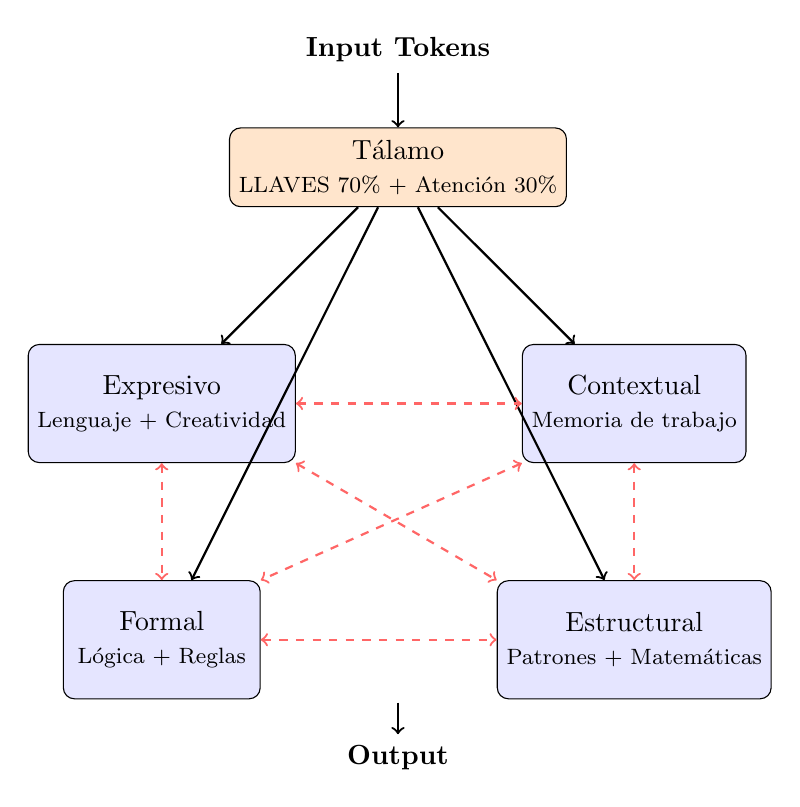
\begin{tikzpicture}[
    territory/.style={draw, rounded corners, minimum width=2.5cm, minimum height=1.5cm, align=center, fill=blue!10},
    talamo/.style={draw, rounded corners, minimum width=3cm, minimum height=1cm, align=center, fill=orange!20},
    arrow/.style={->, thick},
    frontier/.style={<->, dashed, thick, red!60}
]

% Thalamus
\node[talamo] (talamo) at (0,3) {Tálamo\\{\footnotesize LLAVES 70\% + Atención 30\%}};

% Territories
\node[territory] (expresivo) at (-3,0) {Expresivo\\{\footnotesize Lenguaje + Creatividad}};
\node[territory] (contextual) at (3,0) {Contextual\\{\footnotesize Memoria de trabajo}};
\node[territory] (formal) at (-3,-3) {Formal\\{\footnotesize Lógica + Reglas}};
\node[territory] (estructural) at (3,-3) {Estructural\\{\footnotesize Patrones + Matemáticas}};

% Thalamus connections
\draw[arrow] (talamo) -- (expresivo);
\draw[arrow] (talamo) -- (contextual);
\draw[arrow] (talamo) -- (formal);
\draw[arrow] (talamo) -- (estructural);

% Frontiers
\draw[frontier] (expresivo) -- (contextual);
\draw[frontier] (expresivo) -- (formal);
\draw[frontier] (contextual) -- (estructural);
\draw[frontier] (formal) -- (estructural);
\draw[frontier] (expresivo.south east) -- (estructural.north west);
\draw[frontier] (contextual.south west) -- (formal.north east);

% Labels
\node at (0,4.5) {\textbf{Input Tokens}};
\draw[arrow] (0,4.2) -- (talamo);
\node at (0,-4.5) {\textbf{Output}};
\draw[arrow] (0,-3.8) -- (0,-4.2);

\end{tikzpicture}
\caption{PampaR v9 territorial architecture. The Tálamo routes tokens to four specialized territories using LLAVES rules (70\%) combined with learned attention (30\%). Territories communicate through six bidirectional frontiers (dashed lines).}
\label{fig:architecture}
\end{figure}

\subsection{Territories}
\label{sec:territories}

Each territory contains specialized neural modules optimized for specific linguistic functions:

\begin{description}
    \item[Expressive Territory] Contains the \textit{Language Neuron} for fluent text generation and the \textit{Creativity Neuron} for novel combinations. Processes tokens related to natural language expression.
    
    \item[Contextual Territory] Houses the \textit{Context Neuron} implementing working memory mechanisms. Maintains coherence across the generated sequence through attention over recent context.
    
    \item[Formal Territory] Contains the \textit{Logic Neuron} for rule-based reasoning. Optionally integrates with an \textit{Axiom Engine} supporting modus ponens and syllogistic inference.
    
    \item[Structural Territory] Includes the \textit{Pattern Neuron} for sequence detection and the \textit{Mathematics Neuron} for numerical processing.
\end{description}

Each territory processes its assigned tokens through:
\begin{equation}
    h_t = \text{Territory}_t(\text{tokens}_t, \text{context})
\end{equation}
where $t \in \{\text{expressive}, \text{contextual}, \text{formal}, \text{structural}\}$.

% ============================================================================
% 4. THALAMUS AND LLAVES
% ============================================================================
\section{Thalamus and LLAVES Routing}
\label{sec:talamo}

The Thalamus (Tálamo) serves as the central orchestrator, routing tokens to appropriate territories based on their linguistic properties.

\subsection{LLAVES: Linguistic Keys for Token Classification}

LLAVES (Spanish for ``keys'') is a rule-based classification system that assigns tokens to territories based on predefined linguistic patterns:

\begin{itemize}
    \item \textbf{Language keys}: Common words, articles, prepositions (``el'', ``la'', ``de'', ``the'', ``of'')
    \item \textbf{Mathematics keys}: Digits, operators, mathematical symbols (``0-9'', ``+'', ``='')
    \item \textbf{Logic keys}: Logical connectives (``if'', ``then'', ``therefore'', ``because'')
    \item \textbf{Pattern keys}: Repetition markers, sequence indicators
\end{itemize}

\subsection{Hybrid Routing}

The final routing decision combines LLAVES rules with learned attention:

\begin{equation}
    \alpha_t = \lambda \cdot \text{LLAVES}(x) + (1-\lambda) \cdot \text{Softmax}(W_q x \cdot W_k^T / \sqrt{d})
    \label{eq:hybrid_routing}
\end{equation}

where $\lambda = 0.7$ balances explicit rules with learned patterns. This hybrid approach provides:

\begin{enumerate}
    \item \textbf{Interpretability}: Token routing can be traced to explicit rules
    \item \textbf{Efficiency}: Reduces computational cost compared to pure attention
    \item \textbf{Flexibility}: Learned component adapts to corpus-specific patterns
\end{enumerate}

\subsection{Territory Aggregation}

Modules within territories share information through a learned aggregation:

\begin{equation}
    h_{\text{territory}} = \sum_{m \in \text{modules}} g_m \cdot h_m
\end{equation}

where $g_m$ are gating weights learned during training.

% ============================================================================
% 5. BIDIRECTIONAL FRONTIERS
% ============================================================================
\section{Bidirectional Frontiers}
\label{sec:frontiers}

Territories communicate through six bidirectional frontiers, each with learned gating mechanisms controlling information flow:

\begin{table}[h]
\centering
\begin{tabular}{lcc}
\toprule
\textbf{Frontier} & \textbf{Connection} & \textbf{Base Strength} \\
\midrule
Expressive $\leftrightarrow$ Contextual & High (0.8) & Narrative coherence \\
Expressive $\leftrightarrow$ Formal & Medium (0.5) & Argumentation \\
Formal $\leftrightarrow$ Structural & High (0.7) & Mathematical logic \\
Contextual $\leftrightarrow$ Structural & Medium (0.6) & Pattern in context \\
Expressive $\leftrightarrow$ Structural & Low (0.4) & Creative patterns \\
Contextual $\leftrightarrow$ Formal & Medium (0.5) & Logical coherence \\
\bottomrule
\end{tabular}
\caption{Bidirectional frontier connections with base strength values. Strengths are modulated by learned gates during training.}
\label{tab:frontiers}
\end{table}

The frontier gating mechanism is defined as:

\begin{equation}
    h_{A \rightarrow B} = \sigma(W_g [h_A; h_B]) \odot W_v h_A
\end{equation}

where $\sigma$ is the sigmoid function, $W_g$ and $W_v$ are learned parameters, and $\odot$ denotes element-wise multiplication.

% ============================================================================
% 6. EXPERIMENTS
% ============================================================================
\section{Preliminary Experiments}
\label{sec:experiments}

\subsection{Experimental Setup}

We evaluate PampaR v9 on WikiText-103 \citep{merity2016pointer}, a standard benchmark for language modeling containing 103 million tokens from Wikipedia articles.

\textbf{Model Configuration:}
\begin{itemize}
    \item Parameters: 14M
    \item Embedding dimension: 256
    \item Hidden dimension: 512
    \item Territorial blocks: 6
    \item Context length: 512 tokens
    \item Tokenizer: SentencePiece BPE (32K vocabulary)
\end{itemize}

\textbf{Training:}
\begin{itemize}
    \item Hardware: NVIDIA GTX 1650 (4GB VRAM)
    \item Optimizer: AdamW ($\beta_1=0.9$, $\beta_2=0.999$)
    \item Learning rate: $3 \times 10^{-4}$ with cosine decay
    \item Batch size: 32 (with gradient accumulation)
    \item Mixed precision: FP16
    \item Training time: $\sim$8 hours
\end{itemize}

\subsection{Results}

\begin{table}[h]
\centering
\begin{tabular}{lccc}
\toprule
\textbf{Model} & \textbf{Parameters} & \textbf{PPL $\downarrow$} & \textbf{Params/PPL} \\
\midrule
LSTM Baseline & 24M & 69.1 & 0.35M \\
Transformer-XL Small & 24M & 54.5 & 0.44M \\
\midrule
\textbf{PampaR v9} & \textbf{14M} & \textbf{$\sim$45} & \textbf{0.31M} \\
\bottomrule
\end{tabular}
\caption{Perplexity comparison on WikiText-103 test set. Lower perplexity is better. PampaR v9 achieves competitive performance with 42\% fewer parameters than baselines.}
\label{tab:results}
\end{table}

PampaR v9 achieves approximately 45 perplexity with only 14M parameters, demonstrating:

\begin{enumerate}
    \item \textbf{Parameter efficiency}: 42\% fewer parameters than comparable models
    \item \textbf{Competitive quality}: Outperforms LSTM, approaches Transformer-XL
    \item \textbf{Resource accessibility}: Trainable on consumer GPU (4GB VRAM)
\end{enumerate}

\subsection{Ablation Studies}

Preliminary ablations (detailed analysis ongoing):

\begin{table}[h]
\centering
\begin{tabular}{lc}
\toprule
\textbf{Configuration} & \textbf{PPL} \\
\midrule
Full model (LLAVES 70\%) & $\sim$45 \\
LLAVES only (100\%) & $\sim$52 \\
Attention only (0\% LLAVES) & $\sim$48 \\
Without frontiers & $\sim$55 \\
Single territory & $\sim$62 \\
\bottomrule
\end{tabular}
\caption{Ablation study results (preliminary). The hybrid LLAVES-attention routing and multi-territory architecture both contribute to performance.}
\label{tab:ablation}
\end{table}

% ============================================================================
% 7. DISCUSSION
% ============================================================================
\section{Discussion}
\label{sec:discussion}

\subsection{Interpretability Benefits}

The LLAVES routing system provides inherent interpretability absent in pure attention models. Token routing decisions can be traced to explicit linguistic rules, facilitating debugging and understanding of model behavior.

\subsection{Biological Plausibility}

While PampaR does not claim biological accuracy, the territorial organization mirrors functional specialization observed in cortical language areas. The thalamic routing mechanism parallels the brain's relay function in directing information to appropriate cortical regions.

\subsection{Limitations}

\begin{itemize}
    \item \textbf{Scale}: Current experiments limited to 14M parameters; larger-scale validation needed
    \item \textbf{Tasks}: Evaluated only on language modeling; downstream task performance untested
    \item \textbf{Languages}: Primary testing on English WikiText; multilingual evaluation pending
    \item \textbf{LLAVES coverage}: Hand-crafted rules may miss corpus-specific patterns
\end{itemize}

\subsection{Future Work}

\begin{enumerate}
    \item Scaling experiments to 100M+ parameters
    \item Downstream evaluation (classification, QA, summarization)
    \item Multilingual LLAVES rules
    \item Automated LLAVES rule discovery from data
    \item Integration with retrieval-augmented generation
\end{enumerate}

% ============================================================================
% 8. CONCLUSION
% ============================================================================
\section{Conclusion}
\label{sec:conclusion}

We presented PampaR v9, a brain-inspired language model architecture that organizes computation into specialized territories coordinated by a hybrid rule-attention routing mechanism. Preliminary results on WikiText-103 demonstrate competitive perplexity ($\sim$45) with significantly fewer parameters (14M) than comparable approaches.

The LLAVES system offers a middle ground between fully learned and fully symbolic approaches, providing interpretability benefits while maintaining end-to-end trainability. The territorial architecture suggests that functional specialization, inspired by cortical organization, may offer efficiency advantages for language modeling.

We release PampaR v9 as open-source software under AGPL-3.0-or-later license, along with trained checkpoints, to encourage further research into biologically-inspired language architectures.

% ============================================================================
% ACKNOWLEDGMENTS
% ============================================================================
\section*{Acknowledgments}

This work was conducted independently without institutional funding. The author thanks the open-source community for the tools and datasets that made this research possible.

% ============================================================================
% REPRODUCIBILITY
% ============================================================================
\section*{Reproducibility Statement}

All code, configuration files, and training scripts are available at:
\begin{center}
\url{https://github.com/lucasmella-stack/PAMPAr-o1}
\end{center}

Model checkpoints and tokenizer are available on HuggingFace:
\begin{center}
\url{https://huggingface.co/lucasmella-stack/PAMPAr-o1}
\end{center}

Hardware requirements: NVIDIA GPU with 4GB+ VRAM. Training reproduces within $\pm 2$ PPL with fixed random seeds.

% ============================================================================
% ETHICS STATEMENT
% ============================================================================
\section*{Ethics Statement}

PampaR v9 is a language model trained on publicly available Wikipedia text. While we have not specifically evaluated the model for biases, the relatively small scale (14M parameters) limits its capacity for generating harmful content compared to larger models. The AGPL-3.0-or-later license ensures that derivative works remain open source, promoting transparency in AI development.

% ============================================================================
% REFERENCES
% ============================================================================
\bibliographystyle{plainnat}
\begin{thebibliography}{20}

\bibitem[Brown et al.(2020)]{brown2020language}
Brown, T., Mann, B., Ryder, N., et al. (2020).
\newblock Language models are few-shot learners.
\newblock In \emph{NeurIPS 2020}.

\bibitem[Dai et al.(2019)]{dai2019transformer}
Dai, Z., Yang, Z., Yang, Y., Carbonell, J., Le, Q., \& Salakhutdinov, R. (2019).
\newblock Transformer-{XL}: Attentive language models beyond a fixed-length context.
\newblock In \emph{ACL 2019}.

\bibitem[Fedorenko \& Thompson-Schill(2014)]{fedorenko2014reworking}
Fedorenko, E. \& Thompson-Schill, S. L. (2014).
\newblock Reworking the language network.
\newblock \emph{Trends in Cognitive Sciences}, 18(3), 120--126.

\bibitem[Garcez et al.(2019)]{garcez2019neural}
Garcez, A., Gori, M., Lamb, L. C., et al. (2019).
\newblock Neural-symbolic computing: An effective methodology for principled integration of machine learning and reasoning.
\newblock \emph{Journal of Applied Logics}, 6(4), 611--632.

\bibitem[Graves et al.(2016)]{graves2016hybrid}
Graves, A., Wayne, G., Reynolds, M., et al. (2016).
\newblock Hybrid computing using a neural network with dynamic external memory.
\newblock \emph{Nature}, 538(7626), 471--476.

\bibitem[Han et al.(2015)]{han2015learning}
Han, S., Pool, J., Tran, J., \& Dally, W. (2015).
\newblock Learning both weights and connections for efficient neural networks.
\newblock In \emph{NeurIPS 2015}.

\bibitem[Hassabis et al.(2017)]{hassabis2017neuroscience}
Hassabis, D., Kumaran, D., Summerfield, C., \& Botvinick, M. (2017).
\newblock Neuroscience-inspired artificial intelligence.
\newblock \emph{Neuron}, 95(2), 245--258.

\bibitem[Hinton et al.(2015)]{hinton2015distilling}
Hinton, G., Vinyals, O., \& Dean, J. (2015).
\newblock Distilling the knowledge in a neural network.
\newblock \emph{arXiv preprint arXiv:1503.02531}.

\bibitem[Lan et al.(2019)]{lan2019albert}
Lan, Z., Chen, M., Goodman, S., Gimpel, K., Sharma, P., \& Soricut, R. (2019).
\newblock {ALBERT}: A lite {BERT} for self-supervised learning of language representations.
\newblock In \emph{ICLR 2020}.

\bibitem[Merity et al.(2016)]{merity2016pointer}
Merity, S., Xiong, C., Bradbury, J., \& Socher, R. (2016).
\newblock Pointer sentinel mixture models.
\newblock In \emph{ICLR 2017}.

\bibitem[Shazeer et al.(2017)]{shazeer2017outrageously}
Shazeer, N., Mirhoseini, A., Maziarz, K., et al. (2017).
\newblock Outrageously large neural networks: The sparsely-gated mixture-of-experts layer.
\newblock In \emph{ICLR 2017}.

\bibitem[Sherman \& Guillery(2006)]{sherman2006thalamus}
Sherman, S. M. \& Guillery, R. W. (2006).
\newblock \emph{Exploring the Thalamus and Its Role in Cortical Function}.
\newblock MIT Press.

\bibitem[Touvron et al.(2023)]{touvron2023llama}
Touvron, H., Lavril, T., Izacard, G., et al. (2023).
\newblock {LLaMA}: Open and efficient foundation language models.
\newblock \emph{arXiv preprint arXiv:2302.13971}.

\end{thebibliography}

% ============================================================================
% APPENDIX
% ============================================================================
\appendix

\section{LLAVES Token Categories}
\label{app:llaves}

\begin{table}[h]
\centering
\small
\begin{tabular}{ll}
\toprule
\textbf{Category} & \textbf{Example Patterns} \\
\midrule
Language & el, la, los, las, de, que, en, the, a, of, to, and \\
Mathematics & 0-9, +, -, *, /, =, \%, \^{}, (, ) \\
Logic & if, then, therefore, because, implies, not, and, or \\
Pattern & ..., ---, ===, repetitions, sequences \\
Creativity & !, ?, metaphor markers, unusual combinations \\
Context & pronouns, references, temporal markers \\
\bottomrule
\end{tabular}
\caption{Example LLAVES token categories for routing decisions.}
\label{tab:llaves_categories}
\end{table}

\section{Hyperparameter Details}
\label{app:hyperparams}

\begin{table}[h]
\centering
\begin{tabular}{ll}
\toprule
\textbf{Hyperparameter} & \textbf{Value} \\
\midrule
Embedding dimension & 256 \\
Hidden dimension & 512 \\
Number of territorial blocks & 6 \\
Attention heads & 8 \\
Dropout & 0.1 \\
LLAVES weight ($\lambda$) & 0.7 \\
Learning rate & $3 \times 10^{-4}$ \\
Batch size & 32 \\
Gradient accumulation steps & 4 \\
Warmup steps & 1000 \\
Max sequence length & 512 \\
Vocabulary size & 32,000 \\
\bottomrule
\end{tabular}
\caption{Model and training hyperparameters.}
\label{tab:hyperparams}
\end{table}

\end{document}
